\chapter{Application to a dynamically twisted flux tube}

\label{chp:kink_instability_straight}

\graphicspath{{images/kink_instability_straight/}}

\section{Introduction}

In chapter~\ref{chp:kink_instability} the dynamics in a magnetic flux rope which is already linearly unstable to the helical kink instability were investigated. An alternative way to excite the kink instability is to start with an initially straight field and apply twisting motions at the boundaries to create a twisted flux rope which eventually becomes unstable to the kink instability. This kind of dynamic excitation of the kink instability is the focus of this chapter. In addition, a fluting instability is found to be excited prior to the development of the kink instability. To my knowledge, this is the first time a fluting instability in coronal conditions has been studied through 3D numerical simulations. Since the kink instability and associated literature has already been introduced in chapter~\ref{chp:kink_instability}, this introduction focuses on the fluting instability.

The fluting instability arises in magnetised plasmas where the plasma pressure gradient is directed in the same direction as the field line curvature, that is the pressure and magnetic tension forces compete. This is similar to the competition between pressure and gravitational forces which gives rise to the Rayleigh-Taylor instability (RTI), a typical example of an interchange instability, where magnetic field lines are minimally bent and are, instead, exchanged during the evolution of the instability. The ideal fluting instability is another example of an ideal interchange instability, confined to a cylindrical geometry. In a twisted flux tube like a coronal loop, the magnetic curvature is always directed towards the axis so the tube may be unstable to fluting when the pressure decreases outwards from the core. Such a pressure distribution is found in the flux tubes studied here. The appearance of the fluting instability is illustrated by, for example, the pressure contours in figure~\ref{fig:kink_field_line_plots}, where the perturbations follow the pitch of the field.

Although the kink instability has been studied in detail in coronal loop models, I do not know of any coronal studies of the fluting instability. In other solar contexts, interchange instabilities can be found in the form of ballooning modes in arcades~\cite{hoodBallooningInstabilitiesSolar1986}, as the instability which forms tubes of specific size in the photosphere~\cite{bunteInterchangeInstabilitySolar1993} and in the buoyancy of flux tubes~\cite{schuesslerInterchangeInstabilitySmall1984}. The instability is more commonly studied in fusion contexts.

While the stability of the ideal (and resistive) fluting instability has been studied extensively in fusion research~\cite{mikhailovskiiInstabilitiesConfinedPlasma1998,zhengAdvancedTokamakStability2015,wessonHydromagneticStabilityTokamaks1978}, the focus is generally on understanding how a particular plasma device may be stabilised to the instability in particular geometries such as that of the mirror machine~\cite{jungwirthTheoryFluteInstability1965} or in toroidal geometries such as the tokomak~\cite{shafranovFluteInstabilityCurrentcarrying1968}. The resistive interchange instability (the resistive form of the fluting instability) can be excited even when the ideal fluting instability is stabilised. As a result, this has been given significantly more attention~\cite{johnsonResistiveInterchangesNegativeV1967,correa-restrepoResistiveBallooningModes1983}.

While this body of research is useful and applicable in solar contexts, it is mostly limited to the stability and linear development of the instability. More detailed investigations of the nonlinear development is required to understand its importance in the context of coronal dynamics and coronal heating. The experiments described in this chapter provide one such investigation and represent an initial exploration into the nonlinear fluting instability in the solar corona.

\subsection{The fluting instability}

In general, the stability of a cylindrical twisted magnetic flux tube is analysed using perturbations of the form
\begin{equation}
  \label{eq:kink_perturbation}
\xi(r, \theta, z) = \xi(r) e^{i(m\theta + kz)},
\end{equation}
where $m$ and $k$ are the wavenumbers in the $\theta$ and $z$ directions, respectively. The helical kink instability occurs for perturbations where $m=1, k\ne0$ and is the only instability of this form which is a body instability, that is it moves the entire body of the flux tube. Perturbations where $m>1$ are termed fluting or interchange instabilities.

When the magnetic field is sheared, as in a twisted magnetic flux tube, an interchange instability (such as the fluting instability) is confined to a surface where the peaks and troughs follow the shear of the field. That is, the instability is confined to the surface where the perturbation wavevector $(0, m/r, k)$ is perpendicular to the direction of the field which, in an axisymmetric, twisted flux tube, is located at a radius $r$ given by
\begin{equation}
  \label{eq:resonant_surface}
\frac{m}{r} B_{\theta}(r) + kB_z(r) \approx 0.
\end{equation}

The stability of a cylindrical flux tube to perturbations of the form~\eqref{eq:kink_perturbation} is given by the classical Suydam's criterion
\begin{equation}
  \label{eq:suydams_criterion}
\frac{B_z^2 S^2}{4} + 2 r p' > 0,
\end{equation}
where $S = r q'/q$ is a measure of the shear, $q = 2\pi r B_z / L B_{\theta}$ is the safety factor for a flux tube of length $L$ and a dash denotes differentiation with respect to $r$~\cite{mikhailovskiiInstabilitiesConfinedPlasma1998}. This applies to both fluting and kink instabilities although many additional effects such as line-tying are not incorporated into the corresponding linear analysis. The effect of line-tying on the kink instability can be found in~\cite{hoodKinkInstabilitySolar1979}. Where~\eqref{eq:suydams_criterion} is not satisfied, the flux tube may be unstable to perturbations of the form~\eqref{eq:kink_perturbation}. When $m>1$, the perturbations remain local to resonant surfaces given by~\eqref{eq:resonant_surface}.

When the criterion is satisfied and the flux tube is linearly stable, it may still be unstable to non-local perturbations, where the shear and pressure are low enough that interchange perturbations do not need to satisfy~\eqref{eq:resonant_surface}. Additionally, the inclusion of resistivity generally reduces the stabilising effect of the shear, permitting growth of a resistive interchange mode, albeit at a lower rate than that in the ideal case~\cite{mikhailovskiiInstabilitiesConfinedPlasma1998}. It will be found that the ideal linear analysis is sufficient for understanding the fluting instabilities investigated in this chapter since the flux tubes investigated here adequately fail the criterion~\eqref{eq:suydams_criterion}.

While Suydam's condition gives an indication of the stability of a flux tube to a given perturbation, the linear growth rate of the ideal fluting instability $\gamma$ can be found via a stability analysis analogous to that of the Rayleigh-Taylor instability (see~\cite{goldstonIntroductionPlasmaPhysics2020}) and is given by
\begin{equation}
  \label{eq:fluting_growth_rate}
\gamma^2 = \frac{2|\nabla p|}{\rho R_c},
\end{equation}
where $R_c$ is the radius of curvature of the magnetic field. This equation only applies when the pressure gradient and radius of curvature vector are in the same direction, that is the plasma is constrained by a concave magnetic field such that the pressure forces and magnetic tension forces are in competition. In a cylindrical, twisted flux tube, the field is always concave towards the central axis of the tube, so any inwardly directed pressure gradient is unstable to fluting.

Throughout this chapter, the twisted flux tube generated by the drivers has a pressure profile which is axisymmetric, approximately independent of $z$ away from the boundaries at $z=\pm2$, and has a negative gradient, hence $|\nabla p|$ may be written as $-d p/ dr$. Similarly, away from the boundaries, the magnetic field has a negligible $r$ component and little dependence on $\theta$ and $z$, allowing the field to be approximated as $\vec{B} = (0, B_{\theta}(r), B_z(r))^{\text{T}}$, in cylindrical coordinates $(r, \theta, z)$. For a twisted field of this form, the radius of curvature is given by 
\begin{equation}
  \label{eq:radius_of_curvature}
  R_c = \frac{1}{|(\vec{b}\cdot\nabla) \vec{b}|} = \frac{r}{b_{\theta}^2},
\end{equation}
where $\vec{b} = \vec{B}/|\vec{B}|$ is the unit vector in the direction of the magnetic field and $b_{\theta}$ is the component of $\vec{b}$ in the azimuthal direction. These approximations allows the growth rate to be written as
\begin{equation}
  \label{eq:fluting_growth_rate2}
\gamma_{ideal}^2 = \frac{-2p'}{\rho R_c}.
\end{equation}

In contrast to the precise form of the equilibrium state and perturbation studied in chapter~\ref{chp:kink_instability}, this is an experiment where a system is driven and instabilities occur naturally as a result of noise providing a random perturbation. As a result of the driving, the flux tube is not in static equilibrium. Consequently, the stability criterion and linear growth rate presented previously are useful as a guide and approximate comparison, but should not be considered as an appropriate prediction of growth rates or overall stability.

\section{Numerical setup}

The non-dimensionalisation scheme and values are identical to those used in chapter~\ref{chp:kink_instability}. The magnetic field is prescribed as initially straight and uniform,
\begin{equation}
\vec{B} = (0, 0, 1)^{\text{T}},
\end{equation}
in a cube of dimension $[-2,2]^3$. The velocity is set everywhere to $\vec{u} = \vec{0}$, the density to $\rho = 1$, the internal energy to $\varepsilon = 8.67\times 10^{-4}$ (corresponding to a temperature of $10^6$ K). At the boundaries, the magnetic field, density, and energy are fixed to their initial values and the velocity to zero except at the upper and lower boundary where the twisting driver, described below, is prescribed. The spatial derivatives of these variables are also set to zero at the boundaries. The resolution is $512$ grid points per dimension, comparable to the highest resolution kink instability studies of~\cite{hoodCoronalHeatingMagnetic2009} or medium resolution studies of~\cite{barefordShockHeatingNumerical2015}. The switching function employed is the von Mises function~\eqref{eq:switching_function} and the switching parameter is chosen to be $a_0 = 150$, a value sufficiently large to ensure the viscosity is anisotropic throughout the entire domain. 

\begin{figure}[t]
  \centering
  \begin{subfigure}{.49\textwidth}
  \centering
  \includegraphics[width=1.0\linewidth]{u_r.pdf}
  \caption{Radial dependence of driver}
  \label{fig:kink_radial_driver}
  \end{subfigure}
  \begin{subfigure}{.49\textwidth}
  \centering
  \includegraphics[width=1.0\linewidth]{u_t.pdf}
  \caption{Acceleration of driver}
  \label{fig:kink_driver_accel}
  \end{subfigure}
  
  \mycaption{Radial velocity profile $u_r(r)$ and acceleration profile $u_t(t)$ of the driver for parameters $u_0 = 0.15$, $r_d = 5$ and $t_r = 2$.}{}
  \label{fig:kink_driver}
\end{figure}

\todo{fix ylabel of plots}

The flux rope is formed by prescribing a slowly accelerating, rotating flow at the upper $z$-boundary as
\begin{equation}
  \label{eq:null_twisting_profile}
  \vec{u} = u_0 u_r(r) u_t(t) (-y, x, 0)^T,
\end{equation}
where $u_r(r)$ describes the radial profile of the twisting motion in terms of the radius $r^2 = x^2 + y^2$,
\begin{equation}
  \label{eq:radial_twisting_function}
  u_r(r) = u_{r0}(1 + \tanh(1 - r_d r^2)),
\end{equation}
where $r_d$ controls the radial extent of the driver, $u_{r0}$ is a normalising factor, and $u_t(t)$ describes the imposed acceleration of the twisting motion,
\begin{equation}
  \label{eq:ramping_up_function}
  u_t(t) = \tanh^2(t/t_r),
\end{equation}
where the parameter $t_r$ controls the time taken to reach the final driver velocity $u_0$. The functions $u_r(r)$ and $u_t(t)$ are plotted in figure~\ref{fig:kink_driver}. At the lower boundary, the flow is in the opposite direction.

This form of driver allows the system to be accelerated slowly enough that the production of disruptive shocks and fast waves is minimal. It is unavoidable that some waves are produced during the boundary acceleration, however these usefully provide one source of noise which eventually forms a perturbation.

The driver velocity is set to $u_0 = 0.15$, the normalising factor is $u_{r0} = 2.08$, and setting $r_d = 5$ corresponds to a driver constrained to $r<1$ and with a peak velocity at $r\approx 0.38$. The ramping time is set to $t_r = 2$, resulting in an acceleration from $0$ to $u_0$ over approximately $5$ Alfv\'en times. These driver parameters correspond to a peak rotational period of $T_R = 15.92$, the length of time taken for one full turn to be injected by a single driver. Both drivers result in twist being added at a rate of $2\pi$ every $7.96$ Alfv\'en times. The twist profile across the entire flux tube develops in such a way that it is qualitatively similar to that studied in chapter~\ref{chp:kink_instability} by $t\approx 20$, however the length of the flux tubes differs significantly. This configuration produces a $z$-directed tube of increasingly twisted magnetic field that eventually becomes unstable to both the fluting instability and the helical kink instability.

Two pairs of simulations were performed, one pair where the background resistivity is set to $\eta=10^{-3}$ and another where $\eta=10^{-4}$. As in chapter~\ref{chp:kink_instability}, only background resistivity is used. Each simulation pair consists of one simulation using isotropic viscosity and another using the switching model~\eqref{eq:switching_model_simple} with the von Mises switching function~\eqref{eq:switching_function}. The value of viscosity is set to $\nu = 10^{-4}$ in all cases.

\section{Results}

The overall development of both instabilities is broadly similar for the two values of resistivity and is described initially. Focus is then placed on the development of the $\eta=10^{-4}$ cases, comparing the results of the two viscosity models. These cases illustrate the development of the instabilities while showcasing the effect of the viscosity models. Then the differences apparent in the $\eta=10^{-3}$ cases are summarised without a full exploration of the (qualitatively similar) results.

\subsection{Overview of instability development}

\begin{figure}[t]
  \centering
    \begin{subfigure}{0.32\textwidth}
      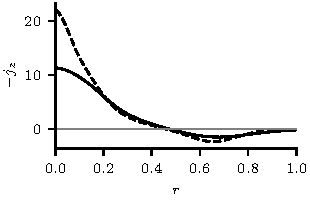
\includegraphics[width=\linewidth]{current_profiles.pdf}
      \caption{Current}
      \label{fig:current_profiles}
    \end{subfigure}
    \hfill
    \begin{subfigure}{0.32\textwidth}
      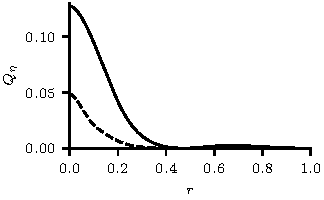
\includegraphics[width=\linewidth]{ohmic_heating_profiles.pdf}
      \caption{Ohmic heating}
      \label{fig:kink_straight_ohmic_heating_profile}
    \end{subfigure}
    \hfill
    \begin{subfigure}{0.32\textwidth}
      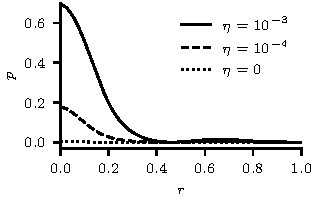
\includegraphics[width=\linewidth]{pressure_profiles.pdf}
      \caption{Pressure}
      \label{fig:pressure_profiles}
    \end{subfigure}
  \mycaption{Gradients in the current density generate pressure gradients through Ohmic heating.}{All plots are from switching cases when $t=20$ through the plane $z=0$. Note the sign of the axial current density $j_z$ has been flipped for comparison and the Ohmic heating is given by $Q_{\eta} = \eta j^2$. The pressure profile of an additional test-case where $\eta=0$ is also shown.}%
  \label{fig:pressure_and_heating}
\end{figure}

In all cases, the initial reaction to the twisting at the upper and lower boundaries is two torsional Alfv\'en waves which travel along the tube from the upper and lower boundaries to the opposite boundary. The interaction between these waves produces an oscillating pattern in the kinetic energy with a period of approximately $4$ Alfv\'en times, equal to the time taken for an Alfv\'en wave to travel the entire length of the domain (visible early in figure~\ref{fig:kink_ke-4}).

As the field continues to be twisted, currents form due to the local shear in the magnetic field which heat the plasma through Ohmic heating. Due to the radial form of the driver, the magnitude of the current density is greatest at the axis of the tube, then decreases radially outwards (figure~\ref{fig:current_profiles}). The orientation of the twisting produces a current directed in the negative $z$-direction for $r\lessapprox0.5$. At $r \approx 0.5$ (corresponding to the radius of peak driving velocity) the current switches direction and is in the positive $z$-direction in a shell where $0.5\lessapprox r \lessapprox 0.8$. This form of twisted field with an inner core of current in one direction surrounded by an oppositely-directed current shell is similar to the prescribed field in chapter~\ref{chp:kink_instability}.

This current profile is reflected in the radial Ohmic heating profile (figure~\ref{fig:kink_straight_ohmic_heating_profile}) and, consequently, in the radial pressure profile (figure~\ref{fig:pressure_profiles}). The highly pressurised core extends to $r\approx 0.2$--$0.4$ (depending on the value of $\eta$) before increasing slightly around $r\approx 0.7$. The secondary bump in pressure is due to the outer shell of current. The pressure gradient near the axis provides the outwardly directed pressure force which competes against the binding action of the magnetic tension to (potentially) result in the fluting instability.  The magnitude of the pressure gradient depends strongly on the value of $\eta$, with lower values producing shallower gradients which (as shall be seen) are more stable to the fluting instability. Indeed, when $\eta=0$, the radial pressure profile is nearly flat and the tube stable to the fluting instability.

In all cases unstable to the fluting instability, it occurs some time between $t=20$ and $t=30$. During this time, the continued driving at the boundaries eventually injects enough twist that the tube also becomes unstable to the kink instability. This initially develops linearly alongside the fluting instability and then erupts during the kink's nonlinear phase, dominating the dynamics and disrupting the fluting instability. The development of the two instabilities is strongly affected by the value of $\eta$ and the viscosity model used.

\subsection{Development where $\eta=10^{-4}$}

\begin{figure}[t]
  \centering
    \begin{subfigure}{0.32\textwidth}
      \includegraphics[width=\linewidth]{swi-4_pressure_13.pdf}
      \caption{$t=26$}
      \label{fig:swi-4_pressure_13}
    \end{subfigure}
    \hfill
    \begin{subfigure}{0.32\textwidth}
      \includegraphics[width=\linewidth]{swi-4_pressure_14.pdf}
      \caption{$t=28$}
      \label{fig:swi-4_pressure_14}
    \end{subfigure}
    \hfill
    \begin{subfigure}{0.32\textwidth}
      \includegraphics[width=\linewidth]{swi-4_pressure_15.pdf}
      \caption{$t=30$}
      \label{fig:swi-4_pressure_15}
    \end{subfigure}
\mycaption{Pressure profiles during the development of the fluting and kink instabilities.}{Shown are slices of pressure through $z=0$ where $\eta = 10^{-4}$ and the viscosity model is switching. Note the difference in colour scale in figure~\ref{fig:swi-4_pressure_15}. The development in the isotropic case is similar.}
\label{fig:kink_pressure_slices-4}%
\end{figure}

\todo{Add inset to pressure figure to properly show bulges in pressure core}

Figure~\ref{fig:kink_pressure_slices-4} shows the pressure profile through $z=0$ where $\eta=10^{-4}$ and the viscosity model is switching for times $t=26$, $28$ and $30$. Around $t=26$ the tube becomes unstable to the $m=4$ fluting instability, when the plasma begins to bulge out diagonally from the high-pressure core (bulges unclear in figure~\ref{fig:swi-4_pressure_13}). As the bulges move radially outwards into lower pressure regions they expand and accelerate, resulting in the entire pressure structure appearing clover-shaped (figure~\ref{fig:swi-4_pressure_14}). By $t=30$ the kink instability has disrupted the fluting instability and is developing nonlinearly (figure~\ref{fig:swi-4_pressure_15}). As is typical of nonlinear kink development, the tube continues to release its stored potential energy as kinetic energy and heat and the contained plasma becomes highly mixed. In the unseen isotropic case, the fluting instability is present but damped, and the kink instability quickly dominates the dynamics.

\begin{figure}[t]
  \centering
    \begin{subfigure}{0.49\textwidth}
      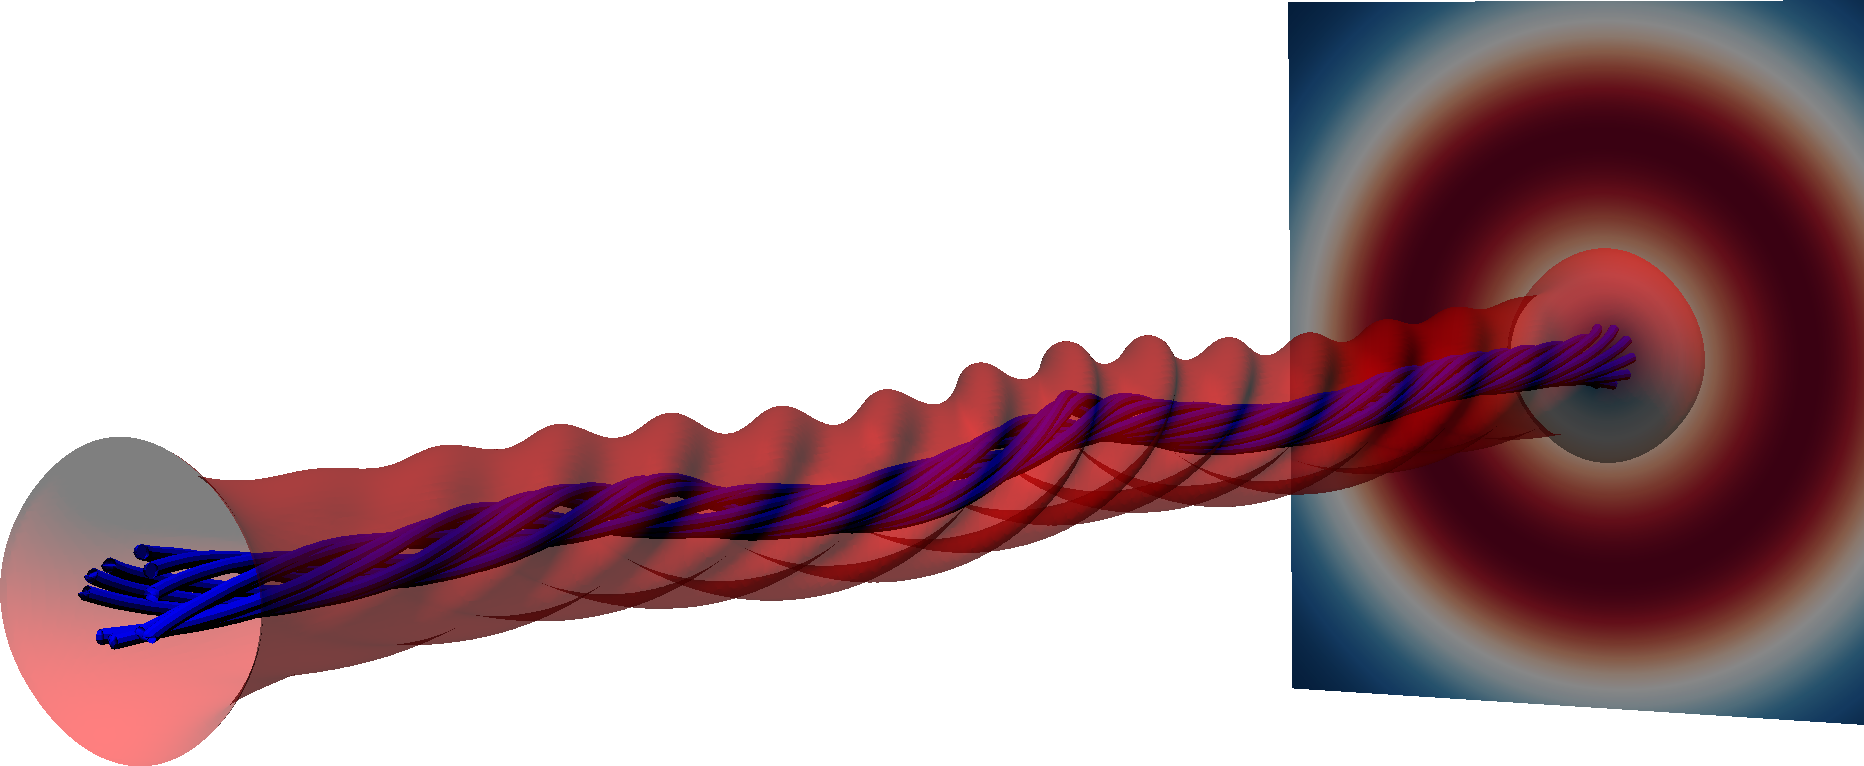
\includegraphics[width=\linewidth]{field_line_plots/cropped/v-4r-4-isotropic_0014_cropped.png}
      \caption{Isotropic}
      \label{fig:field_line_plots_iso}
    \end{subfigure}
    \hfill
    \begin{subfigure}{0.49\textwidth}
      \includegraphics[width=\linewidth]{field_line_plots/cropped/v-4r-4-switching_0014_cropped.png}
      \caption{Switching}
      \label{fig:field_line_plots_swi}
    \end{subfigure}
\mycaption{Simultaneous development of fluting and kink instabilities in the isotropic and switching cases as field lines and pressure contours.}{Field lines and contours of pressure (where $p=0.3$) are plotted at $t=28$. Also shown is the velocity driver as a slice. The fluting instability grows in both cases, though faster in the switching case. The initial stages of the kink instability can also be observed in the field lines of the isotropic case in subfigure~\ref{fig:field_line_plots_iso}.}
\label{fig:kink_field_line_plots}%
\end{figure}

Figure~\ref{fig:kink_field_line_plots} shows the effect the viscosity models have on the initial stages of the fluting and kink instabilities in 3D. While the fluting instability is observed in both cases, it is damped in the isotropic case and grows faster in the switching case. In the latter case, the extended development of the fluting instability appears to disrupt the inner core of field lines and (as shall be seen) slows the growth of the kink instability. In the isotropic case, the fluting instability has been damped to the extent that the kink instability grows uninhibited and quickly disrupts the fluting.

\begin{figure}[t]
  \centering
    \begin{subfigure}{0.49\textwidth}
      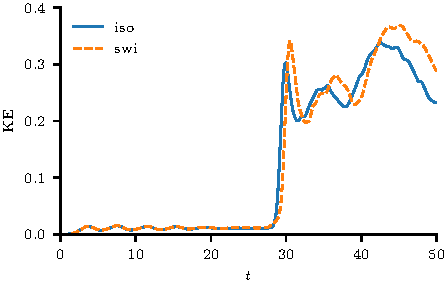
\includegraphics[width=\linewidth]{kinetic_energy-4.pdf}
      \caption{Kinetic Energy}
      \label{fig:kink_ke-4}
    \end{subfigure}
    \hfill
    \begin{subfigure}{0.49\textwidth}
      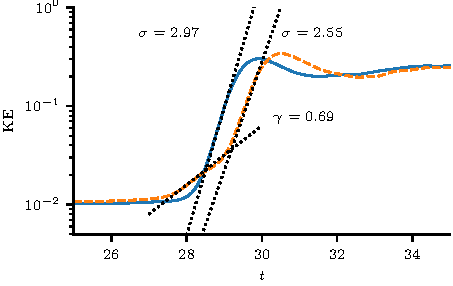
\includegraphics[width=\linewidth]{kinetic_energy_log-4.pdf}
      \caption{Growth rate estimation}
      \label{fig:kink_ke_log-4}
    \end{subfigure}
  \mycaption{Kinetic energy as a function of time showing the development and measured growth rates of the fluting and kink instabilities.}{Both plots are from results where $\eta=10^{-4}$.}
\label{fig:kink_str8_ke-4}%
\end{figure}

Despite the fluting instability appearing in the isotropic case (figure~\ref{fig:field_line_plots_iso}) only in the switching case can the onset of both the fluting and kink instabilities be seen in the kinetic energy profile (figure~\ref{fig:kink_ke_log-4}), where the nonlinear growth rates of the two instabilities are found to be $\gamma = 0.69$ for the fluting and $\sigma = 2.55$ for the kink. The onset times are approximately $t=27$ for the fluting instability and $t=28$ for the kink. In the isotropic case, the growth rate of the kink, $\sigma = 2.97$, is larger than in the switching case, although the onset times appear similar, and the kinetic energy profile shows no evidence of the growth of the fluting instability.

The faster growth of the kink compared to, say, that of chapter~\ref{chp:kink_instability} is due to the relative aspect ratios of the flux tubes. The tube prescribed in chapter~\ref{chp:kink_instability} has an aspect ratio of approximately $20$ compared to the tube studied here which has an aspect ratio of approximately $4$. While the total twist is similar in both tubes (after the drivers have injected twist up to $t\approx20$) the small aspect ratio results in more turns per unit length, resulting in a faster growing instability. The twist per unit length $\Phi = $ also enters into the Suydam criterion~\eqref{eq:suydams_criterion} through the safety factor $q = 2\pi/\Phi$ and predicts a \todo{figure this out}

\begin{figure}[t]
  \centering
    \begin{subfigure}{0.49\textwidth}
      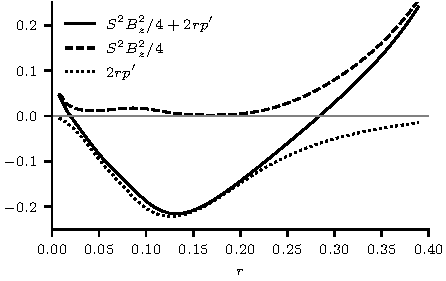
\includegraphics[width=\linewidth]{suydam_condition_4.pdf}
      \caption{Suydam condition}
      \label{fig:suydam_condition_4}
    \end{subfigure}
    \hfill
    \begin{subfigure}{0.49\textwidth}
      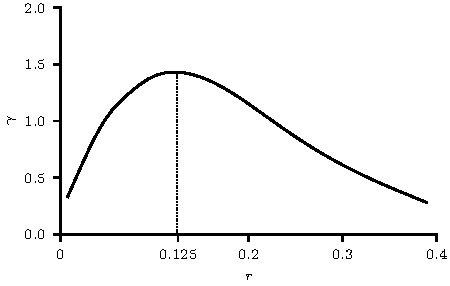
\includegraphics[width=\linewidth]{growth_rate_4.pdf}
      \caption{Linear growth rate}
      \label{fig:growth_rate_4}
    \end{subfigure}
\mycaption{Stability and linear growth rate of the fluting instability.}{In~\ref{fig:suydam_condition_4}, Suydam's stability criterion and contributing terms (LHS of~\eqref{eq:suydams_criterion})  are plotted and in~\ref{fig:growth_rate_4} the predicted linear growth rate~\eqref{eq:fluting_growth_rate2} is plotted. Both plots are produced at $t=20$ for $\eta=10^{-4}$ and using the switching model. The location of the peak linear growth rate is also shown.}
\label{fig:stability_and_growth}%
\end{figure}

Prior to the onset of either instability, the flux tube is found to be linearly unstable to perturbations of the form~\eqref{eq:kink_perturbation} at $t=20$ via Suydam's criterion~\eqref{eq:suydams_criterion} (figure~\ref{fig:suydam_condition_4}). The criterion represents a balance between destabilising pressure gradients and stabilising magnetic shear and in this case, the shear is so small and the pressure gradient so large that the tube is unstable over a wide range of radii, for $ 0.02 \lessapprox r \lessapprox 0.29$. The measure of linear fluting growth rate $\gamma$ is plotted as a function of $r$ at the same time (figure~\ref{fig:growth_rate_4}). While the magnitude of the peak linear growth rate predicts the observed rate reasonably well, the location of the peak growth matches nearly exactly the location of the resonant surface where the observed perturbation grows (figure~\ref{fig:swi-4_pressure_13}).

\begin{figure}[t]
  \centering
    \begin{subfigure}{0.49\textwidth}
      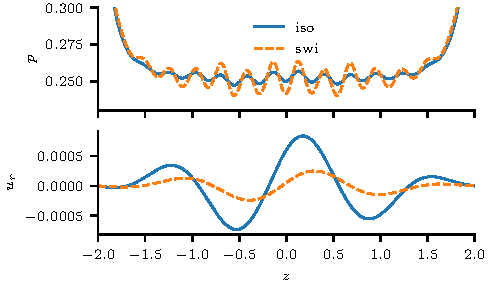
\includegraphics[width=\linewidth]{perturbations_4.pdf}
      \caption{Perturbations}
      \label{fig:pressure_pert_4}
    \end{subfigure}
    \hfill
    \begin{subfigure}{0.49\textwidth}
      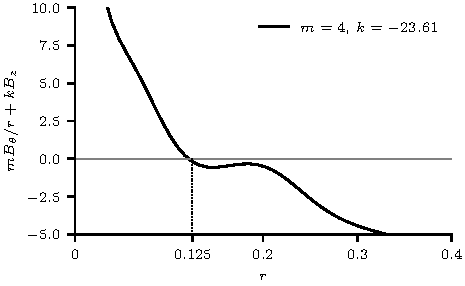
\includegraphics[width=\linewidth]{resonant_surface_4.pdf}
      \caption{Resonance function}
      \label{fig:resonant_surface_4}
    \end{subfigure}
\mycaption{Perturbations corresponding to the fluting and kink instabilities and the spatial radial distribution of the associated resonance function.}{Pressure and velocity perturbations in $z$ (corresponding to the fluting and kink instabilities, respectively) and of the resonance function $m B_{\theta}(r)/r + kB_z(r)$ as a function of $r$ using the observed fluting perturbation wavenumbers. All plots are from snapshots at $t=26$ where $\eta=10^{-4}$ and the viscosity model is switching.}
\label{fig:k_and_resonance}%
\end{figure}

Figure~\ref{fig:pressure_pert_4} plots the observed perturbations corresponding to the fluting and kink instabilities at $t=26$. The fluting perturbation is observed in the pressure and is plotted as a function of $z$ following a line through the point $(r, \theta) = (0.101, 0)$. The kink instability is observed in the $x$-velocity (a proxy for the radial velocity) through the axis. Comparing the magnitudes of the perturbations at this time suggests the fluting instability is close to transitioning to its nonlinear phase while the kink instability is still very much in its linear phase.

The value of $k$ for each perturbation is calculated as $k = 2\pi/\tilde{\lambda}$ where $\tilde{\lambda}$ is the wavelength of the perturbation, measured as the difference between the two peaks closest to $z=0$ (thus minimising the influence of line-tying on the measurement). This gives a value of $k_{flute}=23.61$ and $k_{kink}=4.57$ for both viscosity models. Hence, the observed most unstable fluting perturbation is that of the form~\eqref{eq:kink_perturbation} where $m=4$ and $k=23.61$ and the observed kink instability is that where $m=1$ and $k=4.57$. Using these values, it is observed that the fluting perturbation exactly resonates with the field, that is $m B_{\theta}(r)/r + kB_z(r) = 0$, at $r=0.125$ (figure~\ref{fig:resonant_surface_4}). This is precisely the predicted radius of peak linear growth (figure~\ref{fig:growth_rate_4}). At this time the perturbation is close to resonance, that is $m B_{\theta}(r)/r + kB_z(r) \approx 0$, over a range of radii from $r=0.125$ to $0.2$.

Comparing the effect of the viscous models on the perturbations, in the isotropic case, the fluting perturbation is damped, while in the switching case the kink perturbation is diminished, explaining why the fluting instability appears more readily in the switching case (figure~\ref{fig:kink_ke-4}).

\subsection{Development where $\eta=10^{-3}$}

\begin{figure}[t]
  \centering
    \begin{subfigure}{0.32\textwidth}
      \includegraphics[width=\linewidth]{swi-3_pressure_12.pdf}
      \caption{$t=24$}
      \label{fig:swi-3_pressure_12}
    \end{subfigure}
    \hfill
    \begin{subfigure}{0.32\textwidth}
      \includegraphics[width=\linewidth]{swi-3_pressure_14.pdf}
      \caption{$t=28$}
      \label{fig:swi-3_pressure_14}
    \end{subfigure}
    \hfill
    \begin{subfigure}{0.32\textwidth}
      \includegraphics[width=\linewidth]{swi-3_pressure_15.pdf}
      \caption{$t=30$}
      \label{fig:swi-3_pressure_15}
    \end{subfigure}
    \hfill
    \begin{subfigure}{0.32\textwidth}
      \includegraphics[width=\linewidth]{swi-3_pressure_16.pdf}
      \caption{$t=32$}
      \label{fig:swi-3_pressure_16}
    \end{subfigure}
    \hfill
    \begin{subfigure}{0.32\textwidth}
      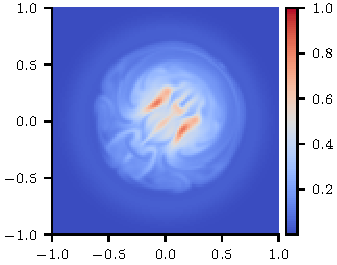
\includegraphics[width=\linewidth]{swi-3_pressure_17.pdf}
      \caption{$t=34$}
      \label{fig:swi-3_pressure_17}
    \end{subfigure}
    \hfill
    \begin{subfigure}{0.32\textwidth}
      \includegraphics[width=\linewidth]{swi-3_pressure_18.pdf}
      \caption{$t=36$}
      \label{fig:swi-3_pressure_18}
    \end{subfigure}
\mycaption{Pressure profiles through $z=0$ during the development of the fluting and kink instabilities in the higher resistivity switching case.}{The viscosity model is switching and $\eta = 10^{-3}$. In contrast to the case of $\eta=10^{-4}$, the nonlinear development of the fluting instability has time to mix the interior of the flux tube before the onset of the kink instability, the growth of which is affected by the mixed plasma.}
\label{fig:kink_pressure_slices-3}%
\end{figure}

Figures~\ref{fig:kink_pressure_slices-3} show the prolonged development of the fluting instability and the slow nonlinear development of the kink. Due to the enhanced Ohmic heating when $\eta=10^{-3}$, the pressure gradient is substantially stronger than when $\eta=10^{-4}$ and the fluting instability is excited much earlier. Compared to the $\eta=10^{-4}$ cases, the instability occurs further from the axis, at $r\approx0.16$, and the larger pressure gradient drives the bulges further from the axis in the nonlinear phase (figure~\ref{fig:swi-3_pressure_12}). These bulges continue to extend outwards and mix the plasma as they develop. The kink instability can be observed moving the axis of the tube diagonally upwards and to the right in figure~\ref{fig:swi-3_pressure_15}. At this time in the $\eta=10^{-4}$ cases, the nonlinear development of the kink was further along (figure~\ref{fig:swi-4_pressure_15}). The development of the kink then proceeds slowly as it moves the axis of the tube through the mixed region to eventually begin the reconnection process with the outer region of field that is typical of the instability in this kind of flux tube (as was observed in chapter~\ref{chp:kink_instability}).

\begin{figure}[t]
  \centering
    \begin{subfigure}{0.49\textwidth}
      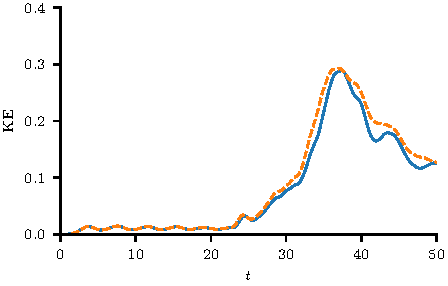
\includegraphics[width=\linewidth]{kinetic_energy-3.pdf}
      \caption{Kinetic Energy}
      \label{fig:kink_ke-3}
    \end{subfigure}
    \hfill
    \begin{subfigure}{0.49\textwidth}
      \includegraphics[width=\linewidth]{kinetic_energy_log-3.pdf}
      \caption{Growth rate estimation}
      \label{fig:kink_ke_log-3}
    \end{subfigure}
\mycaption{Kinetic energy as a function of time in the cases where $\eta=10^{-3}$.}{The results from both viscosity models are shown. The fluting instability appears earlier than where $\eta=10^{-4}$ and the growth rate of the kink instability is decreased.}
\label{fig:kink_str8_ke-3}%
\end{figure}

It is evident from the kinetic energy profile that the fluting instability develops much earlier than in the $\eta=10^{-4}$ cases and grows at an increased rate of $\gamma = 1.06$ (figure~\ref{fig:kink_ke_log-3}). The kink instability grows at a rate of $\sigma \approx 0.15$, much slower than that observed in the $\eta=10^{-4}$ cases, and much lower than the fluting instability. One key observation is that, despite the early and disruptive growth of the fluting instability, the kink instability still generates the bulk of the kinetic energy (figure~\ref{fig:kink_ke-3}).

Due to the influence of the drivers on the kinetic energy, the fluting growth rate is difficult to estimate from the kinetic energy profile as accurately as in the $\eta=10^{-4}$ cases. Since the kink instability occurs after the development of the fluting, its growth rate is similarly difficult to gauge. Nevertheless, it is clear that the fluting instability grows at a rate of the same order as that in the $\eta=10^{-4}$ cases. It is also apparent that the kink instability grows much slower in the $\eta=10^{-3}$ cases.

\begin{table}[]
\centering
\begin{tabular}{ccc}
&
$\eta=10^{-4}$ &
$\eta=10^{-3}$ \\
\midrule
Predicted linear $\gamma$ & 1.43 & 2.72  \\
Observed nonlinear $\gamma$ & 0.69 & 1.06  \\
Observed $\sigma$ & 2.55 & 0.15\\
\midrule
Radius of peak $\gamma$ & 0.125 & 0.163 \\
Observed $r_s$ & 0.125 & 0.163 \\
\midrule
Observed $k_{flute}$ & 23.61 & 16.05 \\
Observed $k_{kink}$ & 4.57 & 4.53 \\
\end{tabular}
\caption{Quantitative differences in the observed perturbations between results for both values of $\eta$. See text for details of measurements times.}
\label{tab:kink_fluting_params}
\end{table}

Table~\ref{tab:kink_fluting_params} summarises the quantitative differences between the results for the two values of $\eta$. All values are calculated from simulations using the switching model with the exception of $k_{kink}$ which is measured from isotropic results due to noise in the switching case (the value of $k_{kink}$ appears similar, however). The results of the isotropic cases are qualitatively similar. The radius of peak $\gamma$ is calculated at time $t=20$. The fluting wavenumber $k$ and observed $r_s$ are measured at times just prior to the nonlinear development of the fluting instability, that is at $t=22$ when $\eta=10^{-3}$ and $t=26$ when $\eta = 10^{-4}$. The kink wavenumber is measured at $t=26$ in both cases. These times allow fair comparison between measurements.

The longitudinal wavenumber $k_{kink}$ of the observed kink perturbation remains similar in both cases since the instability is essentially governed by the twist injected by the driver which remains the same in both cases. In contrast, the longitudinal wavenumber $k_{flute}$ of the observed fluting perturbation is lower in the $\eta=10^{-3}$ cases. This is due to the different resonant surface within which the perturbation grows, the location being dictated by the peak of the linear growth rate. Note that the location of this peak again matches well the location of the observed resonant surface, as in the $\eta=10^{-4}$ cases. Similar to the $\eta=10^{-4}$ cases, the peak growth rate predicted by the linear analysis is the same order of magnitude as the observed growth rate.

\section{Discussion}

Due to the perturbations arising from numerical noise, it is likely that the $m=4$ perturbation is excited due to influences from the boundaries in the Cartesian box, for example through the interaction of reflected fast waves generated in part by the driver. Performing a similar experiment in a cylindrical numerical domain, or prescribing a variety of perturbations in the Cartesian domain may reveal other, faster growing modes. The modes may also be influenced by nonlinear coupling between the $m>1$ and $m=1$ modes, as is found in the study of kink and fluting oscillations~\cite{terradasEffectMagneticTwist2018,rudermanNonlinearGenerationFluting2017a}.

This set of experiments has shown that the mixing as a result of the nonlinear fluting instability appears to slow the growth of the kink instability. In the linear regime it seems unlikely that the linear perturbations of either the fluting or kink are able to directly couple, given that the kink instability generally presents at the axis of a flux tube and the fluting at some resonant surface away from the axis. Further investigation of the nonlinear interaction between the two instabilities is required.

Since the main driver of the fluting instability is the pressure gradient generated through Ohmic heating, it is prudent to ask if the same pressure gradient could be generated using physical coronal values of the resistivity (of approximately $\eta=10^{-8}$~\cite{craigAnisotropicViscousDissipation2009a}) which are much smaller than those studied here. Ohmic heating scales with $\eta j^2$ and not necessarily with $\eta$ itself so, even at realistic values of $\eta$, the current density may be large enough that Ohmic heating is sufficient to generate gradients unstable to the fluting instability in real coronal loops. However, the simulations presented here do not incorporate radiation or thermal conductivity, two processes which would remove energy (and thus pressure) from high-pressure regions in a coronal loop and thus could remove the required conditions for the growth of a fluting instability. Performing a similar experiment with realistic values of the resistivity is currently computationally infeasible, so direct experimentation is unavailable. Instead, performing a parameter study at computationally feasible resistivities with the aim of establishing a scaling law may provide at least an indication of whether Ohmic heating could excite the fluting instability at physical resistivities. Including losses from radiation and thermal conductivity would provide an even stronger indication of whether coronal loops could be unstable to the fluting instability. Regardless of the specific heating mechanism, coronal loops with strong radial pressure gradients have been observed~\cite{foukalTemperatureStructurePressure1975} and such loops may be unstable to the fluting instability. Modelling of a loop where the fluting instability has been excited (but not the kink) would provide a useful comparison to observations.

These results show that a flux tube can be unstable to the fluting instability and yet the faster growing kink instability can quickly dominate when the pressure gradient is small enough. However, the opposite case is also observed, where a faster growing fluting instability appears to slow the growth of the kink instability although, importantly, it does not fully disrupt the development of the kink. Understanding the balance between the nonlinear growth rates of the two instabilities is important in understanding whether the fluting instability may be found at all in the real solar corona, or whether a realistic growth rate is too slow compared to that of the kink instability.

\section{Conclusion}

This chapter details the nonlinear development of two ideal instabilities, the kink and fluting instabilities, both of which develop naturally in the course of twisting an initially straight magnetic flux tube. This provides a different approach to that employed in the simulations performed in chapter~\ref{chp:kink_instability} in that the instabilities are not excited by any prescribed perturbations but, instead, the field is dynamically driven into an unstable state and the perturbations provided by noise in the system. Not only is the kink instability excited due to the twist in the field, a pressure-driven fluting instability can also be excited in unstable pressure gradients generated by Ohmic heating. Simulations were run over two values of resistivity, $\eta=10^{-3}$ and $10^{-4}$, and for two forms of viscosity, isotropic and switching, providing an initial and important first step into the simulation of nonlinear fluting instabilities in the solar corona.

It has been shown that the fluting instability can be quickly dominated by the kink instability if the kink grows substantially faster than the fluting. However, if the fluting has time to develop nonlinearly, it mixes the plasma within the flux tube, generating small scale current sheets and releasing some magnetic energy. The overall effect of this mixing is to slow the growth of the kink instability. The slowed growth of the kink does not appear to impact the total kinetic energy release, only the time over which it is released. 

The form of viscosity has been found to significantly affect the growth of the fluting instability. Importantly, isotropic viscosity is found to damp the growth of the fluting instability to the degree that it is unable to grow appreciably before the onset of the faster growing nonlinear kink instability. Overall, the switching model permits greater release of kinetic energy. Similar to chapter~\ref{chp:kink_instability}, isotropic viscous heating is found to be significantly lower than anisotropic (switching) viscous heating, by approximately two orders of magnitude.

These numerical experiments have provided evidence that the fluting instability can occur in twisted magnetic flux ropes and grow at similar rates to the kink instability. Further estimation of the relative growth rates in more realistic coronal loop setups is required to fully understand if the fluting instability plays a pertinent role in coronal loop physics.
